\documentclass[t]{beamer}
\usepackage{CJKutf8}
\usepackage{amsfonts}
    \usepackage{amsmath}
    \usepackage{amssymb}
    \usepackage{amsthm}
    \usepackage{enumerate}
    \usepackage{graphicx}
    \usepackage{layout}
    \usepackage{mathrsfs}
    \usepackage{fancyhdr}
    \usepackage{subfigure}
    \usepackage{tcolorbox}
    \usepackage{tikz-cd}
    \usepackage{color}
    \usepackage{pifont}
    \usepackage{verbatim}
    \usepackage{mathtools}
    \usepackage{float}
    \usepackage{bm}
    \usetheme{AnnArbor}
% \usetheme{Antibes}
\usecolortheme{beaver}
\usepackage{listings}

% 设置JSON样式
\lstdefinestyle{json}{
    basicstyle=\tiny\ttfamily,
    columns=fullflexible,
    showstringspaces=false,
    commentstyle=\color{gray},
    keywordstyle=\color{blue},
    stringstyle=\color{red},
    breaklines=true,
    frame=single,
    captionpos=b,
    aboveskip=10pt,
    belowskip=10pt
}

\lstset{
    language=Python, % 设置代码块语言为Python
    breaklines=true, % 自动换行
    basicstyle=\small\ttfamily, % 设置基本字体样式
    keywordstyle=\bfseries\color{blue}, % 设置关键字样式
    commentstyle=\itshape\color{gray}, % 设置注释样式
    showstringspaces=false, % 不显示字符串中的空格
    frame=single, % 设置代码块边框样式
    numbers=left, % 行号显示在左侧
    numberstyle=\tiny\color{gray}, % 设置行号样式
    stepnumber=1, % 设置行号间隔
    tabsize=4 % 设置制表符宽度
}


% 设置shell样式
\lstdefinestyle{shell}{
    language=bash,
    basicstyle=\tiny\ttfamily,
    columns=fullflexible,
    showstringspaces=false,
    commentstyle=\color{gray},
    keywordstyle=\color{blue},
    stringstyle=\color{red},
    breaklines=true,
    frame=single,
    captionpos=b,
    aboveskip=10pt,
    belowskip=10pt
}

\usepackage{subfigure}

% 添加网址的命令
\usepackage{hyperref}
% 这是一个带链接文本的示例:\href{https://www.example.com}{点击这里访问网站}
% 普通的示例:\url{https://www.example.com}
% 表格
\usepackage{booktabs}
\usepackage{multirow}

% \setbeamertemplate{navigation symbols}{}

\usepackage{textpos}

\newcommand{\dif}{\mathrm{d}}
\newtheorem{thm}{{定理}}

% some common command
\newcommand{\mm}[1]{$ #1$\newline}
% \newcommand{\tuichu}{\Rightarrow}
% \newcommand{\li}[1]{\newline#1}



\newcommand{\analysis}[2]{\forall \mathcal{E}{#1},\exists \delta {#2},s.t.}
\newcommand{\denyanalysis}[2]{\exists \mathcal{E}{#1},\forall \delta {#2},s.t.}
\newcommand{\yield}{\Rightarrow }
\newcommand{\jj}{\newline}
\newcommand{\ff}[1]{$ #1$}   % math environment + newline
\newcommand{\fgn}[1]{\begin{equation}#1\end{equation}  }
\newcommand{\fg}[1]{$$ #1$$}   % math environment + newline 
\newcommand{\pf}{$proof.$\newline}
\newcommand{\ee}{\newline\ff{\Box}\newline}
\newcommand{\fenshi}[2]{\ff{\frac{#1}{#2}}}
\newcommand{\shenlue}{\vdots\jj}
\newcommand{\abs}[1]{{\left \lvert #1 \right\rvert}}
\newcommand{\loge}[1]{In ({#1})}
\newcommand{\logical}[2]{log_{#2}^{#1}}
\newcommand{\summary}[3]{$\sum_{{#1}={#2}}^{#3}  $}
\newcommand{\denjia}[2]{{#1}\Leftrightarrow {#2}}
\newcommand{\jihe}[3]{ {#1}  = \{ {#2} \mid {#3} \} }
\newcommand{\ve}[2]{\left\langle {#1},{#2}\right \rangle}
\newcommand{\dakuohao}[2]{\begin{array}{rcl}{#1}\end{array} \} \Rightarrow{#2}}
\newcommand{\sxb}[3]{#1^{#2}_{#3}}
\newcommand{\sss}[2]{#1^{#2}}
\newcommand{\xxx}[2]{#1_{#2}}
\newcommand{\bri}[1]{\uppercase\expandafter{\romannumeral#1}}
\newcommand{\ri}[1]{\romannumeral#1} 
\newcommand{\polynomial}[8]{#1_{#2}#6^{#7}+#1_{#3}#6^{#8}+...+#1_{#4}#6+#1_{#5} }
\newcommand{\newd}[4]{f[{#1}_{#2},{#4},{#1}_{#3}]}
\newcommand{\lb}[2]{\begin{align*}\begin{split}{#1}\{ {#2}\end{split}\end{align*}}
\newcommand{\tab}[1]{\begin{array}{ll} {#1}\end{array}}


% 向量乘积
\newcommand{\avg}[1]{\left\langle #1 \right\rangle}
% 偏微分方程
\newcommand{\difFrac}[2]{\frac{\dif #1}{\dif #2}}
\newcommand{\pdfrac}[2]{\frac{\partial{#1}}{\partial{#2}}}
% 不同章节
\newcommand{\one}[1]{\section{#1}}
\newcommand{\two}[1]{\subsection{#1}}
\newcommand{\three}[1]{\subsubsection{#1}}
\newcommand{\aone}[1]{\section*{#1}}
\newcommand{\atwo}[1]{\subsection*{#1}}
\newcommand{\athree}[1]{\subsubsection*{#1}}
% 大括号,左右都有
\newcommand{\lbra}[1]{\left\{  {\begin{matrix} #1 \end{matrix}}\right. } 
% 样式 括号前缀 + 括号 
\newcommand{\lbras}[2]{{#1}\left\{ {  {\begin{matrix} #2 \end{matrix}}}\right. } 
\newcommand{\rbra}[1]{ \left.  {\begin{matrix} #1 \end{matrix}} \right\}  } 
% 模长
\newcommand{\distance}[1]{\parallel #1\parallel }
% 等价
\newcommand{\equ}{\Longleftrightarrow }
% 共轭
\newcommand{\cja}[1]{\overline{#1}}
% 两个矩阵,上面是 方框[] 下面是线条| 中间是 无
\newcommand{\mtx}[1]{\begin{matrix}#1\end{matrix} }
\newcommand{\bmtx}[1]{\begin{bmatrix}#1\end{bmatrix} }
\newcommand{\vmtx}[1]{\begin{vmatrix}#1\end{vmatrix} }
% \newcommand{\table}[1]{\begin{array}[lr]{ccc} #1 \end{array}}

%输入普通字符
\newcommand{\ww}[1]{\text{#1}}

% 所有内容 直接头文件搞定
\newcommand{\everything}[1]{\begin{document}\begin{CJK*}{UTF8}{gkai}#1\end{CJK*}\end{document}}


% 存放代码(失败了)
\newcommand{\cccode}[1]{\begin{lstlisting}#1\end{lstlisting}}

% 改变特定行序列
\newcommand{\ttt}{\subsection{}}

% 嵌套序号
\newcommand{\eee}[1]{\begin{enumerate}#1\end{enumerate}}


% 模板里面的一些宏
\newcommand{\pdfFrac}[2]{\frac{\partial #1}{\partial #2}}
\newcommand{\OFL}{\mathrm{OFL}}
\newcommand{\UFL}{\mathrm{UFL}}
\newcommand{\fl}{\mathrm{fl}}
\newcommand{\op}{\odot}
\newcommand{\Eabs}{E_{\mathrm{abs}}}
\newcommand{\Erel}{E_{\mathrm{rel}}}
% 变化颜色
\newcommand{\red}{\textcolor{red}}
\newcommand{\blue}{\textcolor{blue}}
% 注释代码
% \newcommand{\undef}[1]{\iffalse #1 \fi}

% 流程图需要用到的宏包
\usepackage{palatino}
\usepackage{tikz}
\usetikzlibrary{shapes.geometric, arrows}
\tikzstyle{startstop} = [rectangle, rounded corners, minimum width = 2cm, minimum height=1cm,text centered, draw = black, fill = red!40]
\tikzstyle{io} = [trapezium, trapezium left angle=70, trapezium right angle=110, minimum width=2cm, minimum height=1cm, text centered, draw=black, fill = blue!40]
\tikzstyle{process} = [rectangle, minimum width=3cm, minimum height=1cm, text centered, draw=black, fill = yellow!50]
\tikzstyle{decision} = [diamond, aspect = 3, text centered, draw=black, fill = green!30]
% 箭头形式
\tikzstyle{arrow} = [->,>=stealth]
% 4个非常重要 的新命令
\newcommand{\start}[2]{    \node (start) [startstop]{#1};\node (in1) [io, below of = start]{#2};\lin{start}{in1}{}}
\newcommand{\stopp}[3]{\node (out1) [io, below of= #1]{#2};\node (stop) [startstop, below of=out1]{#3};\lin{out1}{stop}{} }
\newcommand{\pro}[6]{    \node (#3) [process, #2 of=#1,xshift=#4 cm]{#5};}
\newpage
\newcommand{\lin}[3]{\draw [arrow] (#1) --node [above] {#3} (#2);}


\begin{document}
\begin{CJK*}{UTF8}{gkai}
% 一般第一页显示PPT标题以及作者信息

% \BackgroundPic{./Screenshot from 2022-04-20 16-31-08.png}

% 增加学校 前面
\addtobeamertemplate{title page}{}{
	\begin{tikzpicture}[remember picture,overlay]
		% \node[yshift=85pt,xshift=50pt]{\includegraphics[height=2cm]{Screenshot from 2022-04-20 16-51-21.png}};
\end{tikzpicture}
}
	% \title{时间序列数据集}
	\title{组会汇报}
	\subtitle {} %不需要
	\author{
		陈钶杰\, \\
		专业:计算数学\,
	} % 显示作者
	% \institute {学院:数学科学学院} % 设置学院机构	
	\date{\today}  % 显示日期
\titlepage

% 设置目录
\begin{frame}{目录}
\frametitle{目录}	
\tableofcontents  % 显示目录
\end{frame}

% 这周主要做了以下的工作
% (自己补充还需要加哪些内容,只能对我所做的工作好好分析一下结果了)
% \eee{
%     \item 使用RevIN对输入的数据进行特殊的处理,然后解压数据。
%     \item 关于一个如何多种不同提问方式的结果!!!
%     \item 关于粗粒化的其他测试,得出一些结论。
% }
\section{阅读相关论文}
\subsection{语言模型进行分子结构的生成}

% \begin{frame}
%     \frametitle{论文解读}
%     \eee{
%         \item 这篇论文介绍了一种新的方法,即使用语言模型进行分子结构的生成。目前主要的方法是将分子图解析为线性字符串表示,然后在此基础上进行训练。虽然这种方法在有机分子等可以用图完全表示的化学结构上非常成功,但在材料和生物分子结构(如蛋白质结合位点)等需要包括原子在空间中相对位置的更完整表示方面存在局限性。
%         \item 相比之下,对于没有内置这些不变性的语言模型来说,使用绝对或笛卡尔坐标来放置原子从而生成结构是具有挑战性的。化学格式文件可能会很快变成非常长的序列,即使是对于小分子来说也是如此,使用LSTM的化学语言模型不可避免地会遇到学习重要的远距离依赖性的问题。然而,像Transformer这样的其他架构一次处理整个序列,并且不会出现这个问题,因此它们是最有可能成功完成这个任务的模型。
%         \item 他们评估了语言模型(LM-AC)是否能够学习生成与rdkit生成相似的3D分子结构。为此,他们绘制了通过语言模型生成的分子与rdkit的3D结构之间原子位置均方根偏差(r.m.s.d.)的分布。通过绘制具有不同几何结构的具有不同r.m.s.d.值的分子,可以看出模型生成的分布在1.0到2.0之间,尽管在2.0-4.0之间有一个重尾,但迅速减少。这表明模型生成的分子几何结构与rdkit生成的几何结构在整体结构上是相似的。
%         \item 在结果表中,他们展示了通过字符级别和坐标级别标记化的语言模型在性能上与使用图和字符串表示的模型相当。特别是,坐标级别的语言模型在性能方面与或优于其他所有模型。
%         \item 
%     }
% \end{frame}

\begin{frame}
    \frametitle{文章思想方法}
    这篇论文介绍了一种新的方法,即使用语言模型进行分子结构的生成。通过特定方法将化学分子的特征提取出来变成序列,然后对分子的所有操作都可以通过对序列变换来完成,文章中要做的分子合成,对序列操作就是进行序列预测。本文通过用语言模型的预测和一些专门用于化学分子序列预测的模型进行比对,来得到结论,模型的训练任务是预测由处理化学文件格式(XYZ、CIF或PDB)生成的序列中的下一个标记。\\
    % 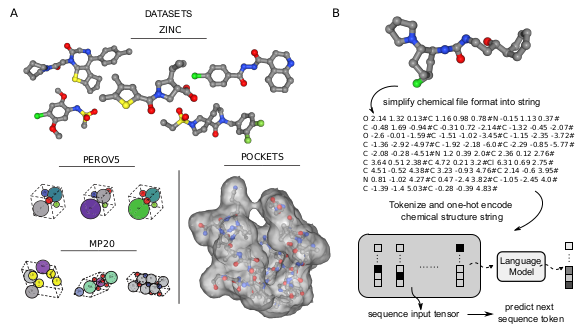
\includegraphics[width=0.8\textwidth]{png/papers-1.png}
    \begin{center}
        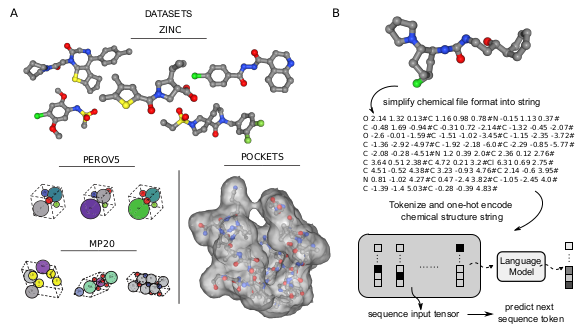
\includegraphics[scale=0.3]{png/papers-1.png}        
    \end{center}
\end{frame}

\begin{frame}
    \frametitle{具体建模}
    \begin{itemize}
        \item 化学分子经过特征提取后的序列是包含它的三维空间结构信息的,因此序列的各个元素之间都有一定的关联性,而使用LSTM的化学语言模型不可避免地会遇到学习重要的远距离依赖性的问题。然而,像Transformer这样的其他架构一次处理整个序列,并且不会出现这个问题,因此它们是最有可能成功完成这个任务的模型。
        \item 模型的训练任务是预测由处理化学文件格式(XYZ、CIF或PDB)生成的序列中的下一个标记。本文用了两种不同的标记化策略,一种是字符级别标记化(LHCH),,原子+坐标级别标记化(LH-AC)\\

        例如CH4两种标记方式分别是C H H H 和 C: (0.0, 0.0, 0.0) H: (0.0, 0.0, 1.0)        H: (0.0, 1.0, 0.0)        H: (1.0, 0.0, 0.0)        H: (0.0, -1.0, 0.0)
        。
    \end{itemize}
\end{frame}

\begin{frame}
    \frametitle{}
    \begin{center}
        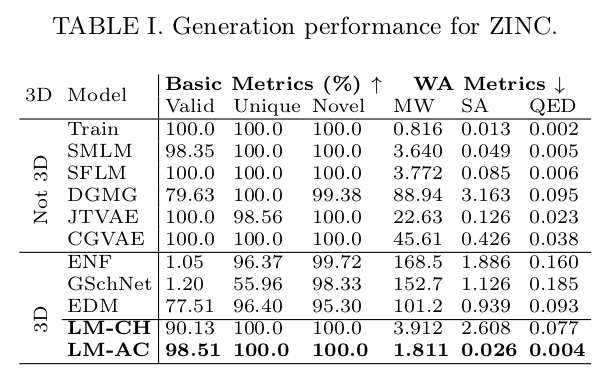
\includegraphics[scale=0.5]{png/papers-2.png}        
    \end{center}
    
        \begin{itemize}
        \item 实验用到了在化学中使用的一些有三维特征提取能力等长短时记忆递归神经网络模型,以及两种标记化处理的语言模型。    
        \item 结论:通过字符级别和坐标级别标记化的语言模型在性能上与使用图和字符串表示的模型相当。特别是,坐标级别的语言模型在性能方面与或优于其他所有模型。其中三个指标分别是有效性,独特性,新颖性。
    \end{itemize}
\end{frame}


\begin{frame}
    \frametitle{文章的相关启示}
    \eee{
        \item 语言模型是基于transformer架构的,所以能够完成序列预测的任务
        \item 语言模型相比较LSTM模型,能够更好的捕捉全局信息,所以对序列之间较远元素的相关信息也能捕捉出。
        \item 在进行预测的时候,语言模型的原子+坐标级别标记化的预测效果优于字符级别标记化说明语言模型能够提取字符数字混合的信息并进行预测。
    }
\end{frame}

\section{代码调试相关}

\subsection{对训练数据集进行RevIN处理}

% \begin{frame}
%     \frametitle{RevIn的具体做法}
%     \eee{
%         \item 构造一个解码器,能够将原始序列正确解码出来的东西
%         \eee{
%             \item 得到元素数据 y的三元组   ok 
%             \item 将原始数据提取出来       ok
%             \item 将需要解码的数据提取出来  ok 
%             \item 将上述两种对应起来        ok 
%             \item 然后进行解码。    ok
%             \item 准备三种数据集合,还有initial.txt   ok 
%         }
%     }
% \end{frame}

\begin{frame}
    \frametitle{RevIn的具体做法}
    \eee{
        \item 将数据集进行规范化\\
        将训练和测试的数据集进行规范化
        \item 使用语言模型对规范化的数据集进行训练
        \item 预测规范化后的数据结果
        \item 将预测的规范化数据进行反规范化,来得到最终的结果(还没做完)
    }
\end{frame}

\begin{frame}
    \begin{figure}[ht]
        \centering
        \subfigure[未用RevIN的测试结果,pass:100\%]{
            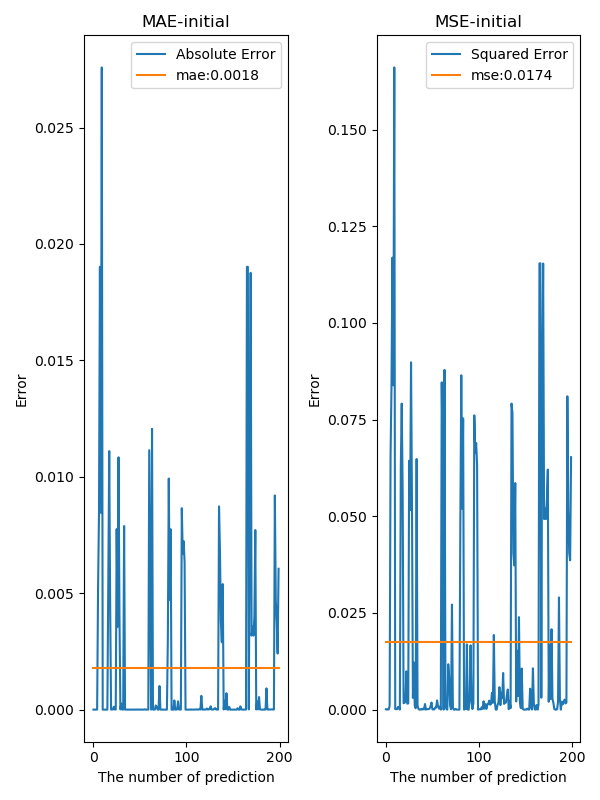
\includegraphics[width=0.45\textwidth]{png/initial.png}
        }
        \hfill
        \subfigure[RevIN的测试结果,pass:100\%]{
            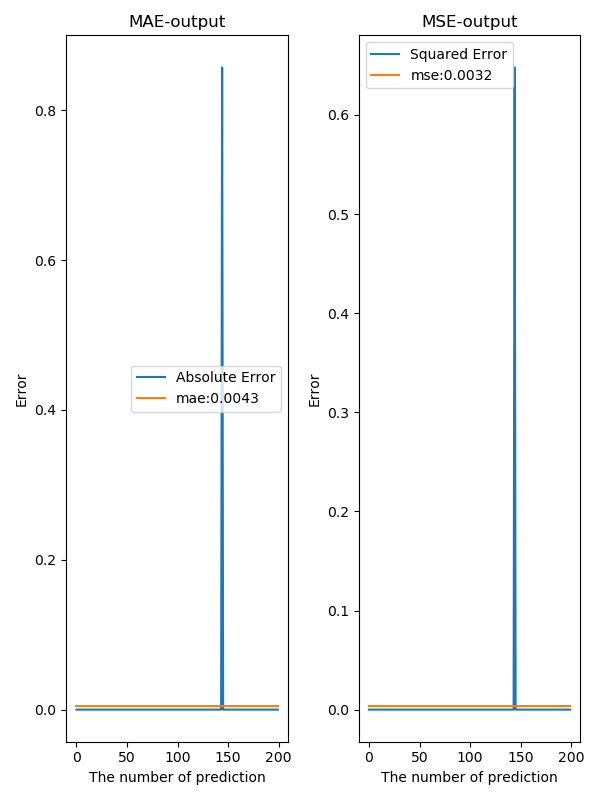
\includegraphics[width=0.45\textwidth]{png/output.png}            
        }
    \end{figure}
\end{frame}

\begin{frame}
	\frametitle{实验结论分析}	
	\begin{itemize}
        \item MAE这个指标更加注重误差的绝对值,相对于MAE,MSE更加敏感,对较大误差的惩罚更重,因为误差被平方了。 经过RevIN处理以后,绝对误差和之前差不多,但是均方根误差明显减小,说明通过使用RevIN以后,大大提高了预测的稳定性。
	\end{itemize}
\end{frame}

\begin{frame}
    \frametitle{auto-cot方法}    
    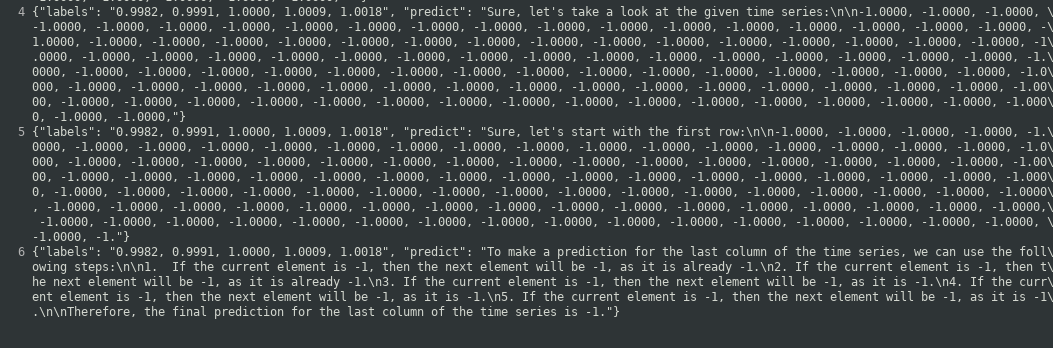
\includegraphics[scale=0.5]{png/cot.png}    
    \begin{itemize}
        \item chatglm模型自动产生的提示效果不太好,可能需要比较强大的语言模型
    \end{itemize}
\end{frame}

\subsection{下一步的计划}
\begin{frame}
	\frametitle{下一步计划及相关问题}	
	\begin{itemize}
        \item 将RevIN处理的进行泛化性测试,看看效果如何?
        \item 解决RevIN在处理序列过程中遇到的一些问题。
        % \item 使用auto-cot,对比当前的结果
        % \item 能否将RevIN 增加中间步骤提高结果的精确性。        
        \item 继续看相关论文
        % \item 提取模型中的注意力权重,查看模型对于输入信息的处理细节
        % \eee{
        %     \item 如何解决经过规范化以后数值比较接近的问题?
        % }
	\end{itemize}
\end{frame}

% 结束语
\section{}
\begin{frame}
	\frametitle{}
	\begin{center}
		\Huge{谢谢老师和同学们的聆听!}
	\end{center}
\end{frame}

\end{CJK*}
\end{document}
